\part{Towards Highly Miniaturized LED Power Systems }
\label{ch:twrd_HMLED}

\chapter{The new coming LED based lighting industry}

The appearance of light in the beginnings of the 19th century and the posterior commercialization was clearly a remarkable fact of the past history. The light bulbs contributed in two major facts that impacted peoples life . First, they enabled to have clear, reliable and safe source of light at home, extending our activity hours longer than the natural sun light. As a matter of fact we can not live without the use of artificial light.   Second, the necessity of electric power helped to develop the first electric power distribution systems. Actually, that fact can be still evidenced since people, generally our grand parents, often use the word \emph{light} when they actually are refereing electricity.

\begin{figure}[!h]
\centering
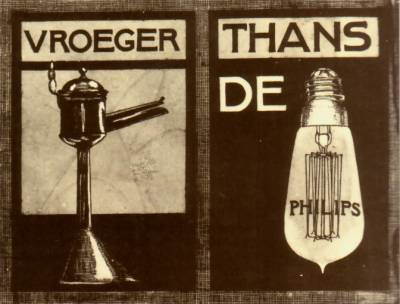
\includegraphics{./0_intro/img/1900-philips3.jpg}
\label{fig:incandescent_light_blub}
\caption{Early incandescent light bulb}
\end{figure}


From the first incandescent light bulb, the lighting industry has not had any big disruptive change to our perception of lighting till the last decade with the apparition of the LED lamps. Besides as many of us thing, it has been done a large effort to improve the efficiency of the light sources while keeping a the quality of the light as good as the incandescent light bulb. Being the florescent lamps one of the biggest contributions during the past century, beginning  to be commercialized around 1930. Later becoming a disruptive change in the lighting market with the introduction the low consumption lamps where Philips was one of the first player launching to the market the first screw-in fluorescent lamp. Although the prices of these lamps has been dropping to become commercially attractive for the costumers, their poorer color rendering factor and the longer setting time compared to the incandescent lamps prevented this lamps to be one-to-one replacement. Therefore the lighting industry has been keep without not too much attention till the introduction the LED based lamps.

\begin{figure}[!h]
\centering
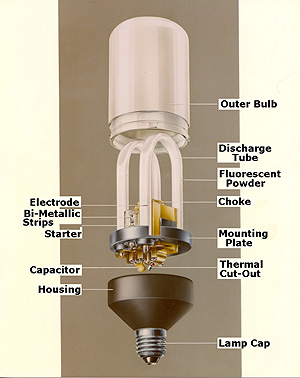
\includegraphics{./0_intro/img/phil1b.jpg}
\label{fig:philips_sl}
\caption{Components of the Philips SL compact fluorescent lamp. }
\end{figure}

The discovery of the high-efficiency blue LED ~\cite{94Nakamura} by Shuji Nakamura in 1994 enabled the quick development of the fist efficient withe LED. These early high power LEDs demonstrated that LEDs where a suitable technology for illumination. The relevance of Nakamura's work has been recognized last year being him awarded with the 2014 Nobel prize in physics. Looking farther we can also confirm the relevance of his invention since the apparition of the LED lamps, lighting is impacting again in our everyday life by changing our traditional concept of luminaries and lighting possibilities. 

\begin{figure}[!h]
\centering
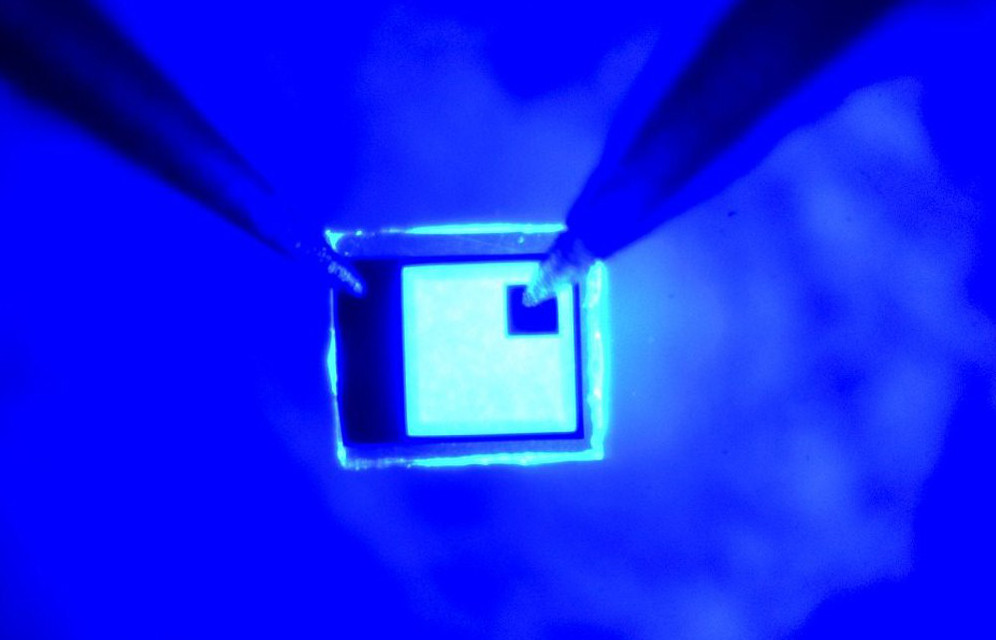
\includegraphics{./0_intro/img/10-7-14-nobel-prize-blue-led.jpg}
\label{fig:philips_sl}
\caption{Picture of a blue laser LED researched by Shuij Nakamura.}
\caption*{Source: \url{http://www.newsweek.com/how-blue-led-changed-world-and-won-nobel-prize-275977} }  
\end{figure}

LED based lamps created a frenetic rush in the lighting industry into bring that technology to the end consumers. Actually the advantages of the LED based lighting, or also known as Solid State Lighting (SSL), are so relevant that in the close future they will replace any of the present lighting technology, that movement has been already named as the \emph{LEDification}. The advantages of SSL are:
\begin{description}
  \item [Efficiency] The light generation inside an LED is produced by the direct mechanism of hold-electron recombination, the supplied energy is a better use of the energy compared to the incandescent lamps. The power consumption can be up to an order of magnitude lower of an incandescent light. 
  
  \item [Size] LEDs are tiny and flat devices, which can be considered as 2-D elements and do not need any vacuum chamber to work. They are much more flexible devices to assembly, and can easily replace the old glass made bulb design.
       
  \item [Color] LED light has a very narrow light spectrum, that can be used to produce directly colored light. Colored lights are becoming more popular in domestic homes becoming a piece of decoration or mood tweaking device.
      
  \item [Dynamics] Compared to any of the traditional sources of light LEDs have no dynamics, actually they have but it's very fast and not appreciable to the human eye. Therefore they do not have any setting time when turned on, which is not the case of CFL. The fast dynamics allows to modulate the light and transmit data without disturbing the human beings.
      
  \item [Lifetime] Solid State devices do not wear off, there fore they can be considered to have an infinite lifetime. In practice LEDs make use of organic phosphores, thus the light quality derates with the use, but the life expectancy of the LED is rated from 20.000 - 100.000 hours being 20 to 100 times longer that the classical light bulbs.  
  
\end{description}
 

This section will make a little dissertation about what is the way to go:
\begin{enumerate}
  \item Cost driven driver production the cheapest the better
  \item Miniaturization + smart driver integration
\end{enumerate}

this section should gasp the current efforts done in order to introduce the LED light to the market. And say that the present way is retrofitting.

The section should close facing the dilemma that once the retrofitting is done where it will be the new market cases, and point that highly integrated drivers
can be one of the possible scenarios where integration and connectivity are part of a single solution.

%\chapter{An overview in LED driving}
%\section{DC-DC Drivers}
%\section{AC-DC Drivers}

\chapter{Introducing switched capacitors in LED drivers}
Presenting the concept of using a SCC with an inductor in order to enable integration and reduction in the size of the inductor.



